\section{Administración de riesgos en un proyecto civil}

Existen tres categorías más importantes en la identificación de riesgos de proyectos IOC:
\begin{itemize}
    \item Riesgos de diseño
    \item Riesgos externos
    \item riesgos ambientales
    \item Riesgos organizacionales
    \item riesgos de administración de proyectos
    \item Riesgos legales y contractuales
    \item Riesgos de construcción
\end{itemize}

Estos riesgos se califican en función de su probabilidad de ocurrencia (del 1 al 5) y su impacto en el proyecto (del 1 al 5). La matriz de riesgos es una herramienta comúnmente utilizada para visualizar y priorizar estos riesgos.
A continuación, se presenta un ejemplo de una matriz de riesgos:
\begin{figure}[h]
    \centering
    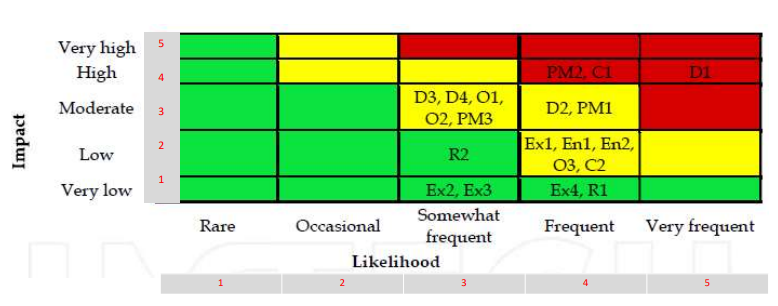
\includegraphics[width=0.8\textwidth]{Graficos/matriz.png}
    \caption{Matriz de riesgos de un proyecto IOC}
    \label{fig:matriz_riesgos}
\end{figure} 

Algunos ejemplos de riesgos que pueden surgir en un proyecto IOC son:
\begin{itemize}
    \item Riesgos de diseño: cambios en los requisitos del cliente, errores de diseño, falta de experiencia del equipo de diseño.
    \item Riesgos externos: cambios en la legislación, problemas con proveedores, condiciones climáticas adversas.
    \item Riesgos ambientales: contaminación del sitio, impacto en la fauna y flora local, problemas de salud pública.
    \item Riesgos organizacionales: falta de comunicación entre departamentos, conflictos internos, falta de recursos.
    \item Riesgos de administración de proyectos: falta de planificación adecuada, problemas con el cronograma, sobrecostos.
    \item Riesgos legales y contractuales: disputas contractuales, incumplimiento de normativas, problemas legales con terceros.
    \item Riesgos de construcción: accidentes laborales, problemas con subcontratistas, retrasos en la entrega de materiales.
\end{itemize}

También se puede hacer una matriz de evaluación de riesgos, que considera 7 factores:
\begin{itemize}
    \item Riesgo
    \item Repercusiones
    \item Probabilidad de que suceda
    \item Magnitud de las repercusiones
    \item Disparador de la acción 
    \item Responsable
    \item Plan de respuesta
\end{itemize}

Un ejemplo de matriz de evaluación de riesgos es el siguiente:
\begin{table}[h]
    \centering
    \small % Reduce tamaño de fuente
    \begin{tabularx}{\textwidth}{|c|X|c|c|X|c|X|}
        \hline
        \textbf{Riesgo} & \textbf{Repercusiones} & \textbf{Probabilidad} & \textbf{Magnitud} & \textbf{Disparador} & \textbf{Responsable} & \textbf{Plan de respuesta} \\
        \hline
        Clima adverso & + costos y retrasos & 3 & 4 & Pronóstico met. 2 días antes & Jefe de obra & Planificación de contingencias y ajustes al cronograma \\
        \hline
    \end{tabularx}
    \caption{Matriz de evaluación de riesgos}
\end{table}

Para poder calcular el riesgo se utiliza la siguiente fórmula:
\begin{equation}
    \text{Riesgo} = \text{Probabilidad} \times \text{Impacto}
\end{equation}
Si un riesgo tiene poca probabilidad y bajo impaccto, será capaz de aceparlo, pero si tiene alta probabilidad y alto impacto, se deberá prestar atención.

\section{Análisis de licitaciones, bases técnicas y contratos}

\subsection*{Etapa Inicial de un Proyecto OOCC}

\begin{itemize}
    \item Garantizar que el contratista/subcontratista comprenda los riesgos al hacer una oferta para un proyecto/servicio propuesto.
    \item El contratista/subcontratista puede incluir cantidades de reserva para contingencias en el precio de la oferta.
    \item El contratista/subcontratista puede desistir de presentar una oferta.
\end{itemize}

\subsection*{Criterios de Presentación de Presupuesto}

\begin{itemize}
    \item La oferta final se puede ver afectada por la estrategia que se haya tomado para la propuesta específica.
    \item El monto final puede bajar si el contratista tiene mucho interés en ganar el proyecto.
    \item El monto final puede subir si se tiene mucho trabajo en paralelo a este proyecto.
\end{itemize}

\subsection*{Decisión para Desarrollar una Propuesta}

\begin{itemize}
    \item La evaluación del contratista sobre la posibilidad de seguir o no con la preparación de una propuesta, en ocasiones se conoce como: \textbf{Decisión de Oferta / No Oferta}.
    \item Se pueden considerar los siguientes factores al decidir desarrollar una propuesta:
    \begin{itemize}
        \item Nuestras ventajas, fortalezas o capacidades diferenciadoras.
        \item Nuestras debilidades.
    \end{itemize}
\end{itemize}

\subsection*{Disminución / Mitigación de Riesgos}

\begin{itemize}
    \item Se pueden considerar los siguientes factores al decidir desarrollar una propuesta:
\end{itemize}

\begin{table}[h]
    \centering
    \small
    \begin{tabular}{|c|p{8cm}|c|p{4cm}|}
        \hline
        \textbf{N°} & \textbf{Factor} & \textbf{Puntuación (A/M/B)} & \textbf{Comentarios} \\
        \hline
        1 & Competencia & & \\
        \hline
        2 & Riesgo & & \\
        \hline
        3 & Consistencia con nuestra misión & & \\
        \hline
        4 & Oportunidad para ampliar nuestras capacidades & & \\
        \hline
        5 & Reputación con el cliente & & \\
        \hline
        6 & Disponibilidad de fondos & & \\
        \hline
        7 & Recursos disponibles para preparar propuesta de calidad & & \\
        \hline
        8 & Recursos disponibles para realizar el proyecto & & \\
        \hline
    \end{tabular}
    \caption{Planilla tipo de Lista de verificación de licitar/no licitar}
\end{table}

\noindent El \textbf{contratista} decidirá la acción de presentar su oferta:

\begin{center}
    \fbox{\textbf{Licitar \quad / \quad No Licitar}}
\end{center}

\subsection*{Factores que Influyen en la Decisión de Licitar / No Licitar}

\noindent Según un estudio, existen tres principales características de factores contribuyentes a la determinación final para licitar o no licitar en la industria de la construcción:

\begin{enumerate}
    \item Factores relacionados a la empresa,
    \item Factores relacionados al proyecto,
    \item Condiciones y expectativas del mercado, junto con consideraciones estratégicas.
\end{enumerate}

\noindent Estos factores pueden ser identificados:
\begin{itemize}
    \item Por el cliente, durante la etapa de elaboración de normativa o el llamado a propuesta (FRP) del proyecto.
    \item Por el contratista, durante la etapa de elaboración de su propuesta.
\end{itemize}

\noindent El \textbf{MANDANTE} decidirá acción de:
\begin{center}
    \fbox{\textbf{Adjudicar \quad / \quad No Adjudicar}}
\end{center}
